				%%%% patron de format latex pour rfia 2000.
				%%%% sans garanties. Plaintes \`a envoyer \`a \dev\null.
				%%%% deux colonnes pas de num\'erotation et 10 points
				%%%% necessite les fichiers a4.sty french.sty et rfia2000.sty
				
				%%%% Pour \LaTeXe
				\documentclass[a4paper,twoside,french]{article}
				\usepackage{rfia2000}
				\usepackage[T1]{fontenc}
				\usepackage[francais]{babel}
				\usepackage[utf8]{inputenc}
				\usepackage{lmodern}
				\usepackage[noend]{algpseudocode}
				\usepackage{subcaption}
				\usepackage{subfig} 
				\usepackage{usual}
				\usepackage{graphicx}
				\usepackage[rflt]{floatflt}
				\pagestyle{plain}
				
				\begin{document}
				%%%%%Pas de date
				\date{}
				%%%%% Titre gras 14 points
				\title{\Large\bf Réparation de plans dans les HTNs réactifs en utilisant la planification symbolique
				       }
			
				\author{\begin{tabular}[t]{c@{\extracolsep{6em}}c@{\extracolsep{6em}}c}
				%%%% pour quatre auteurs
				%%%%\author{\begin{tabular}[t]{c@{\extracolsep{4em}}c@{\extracolsep{4em}}c@{\extracolsep{4em}}c}
				%%%%pour plus d\'ebrouillez-vous !
				Lydia Ould Ouali${}^1$  & Charles Rich${}^2$ & Nicolas Sabouret${}^1$\\
				\end{tabular}
				{} \\
				 \\
				${}^1$        LIMSI-CNRS, UPR 3251, Orsay, France \\
									Univ. Paris-Sud, Orsay, France \\
				${}^2$        	Worcester Polytechnic Institute\\ Worcester, MA, USA\\
				{} \\
				 \\
				 ouldouali@limsi.fr \\
				%Mon adresse complète \\
				%Mon adresse électronique
				}
				\maketitle
				%%%%  Pas de num\'erotation sur la page de titre
				\thispagestyle{empty}
				\subsection*{R\'esum\'e}
				Construire des modèles formels pour planifier les prochaines actions d'un agent est un problème crucial en Intelligence Artificielle. Dans ce travail, nous proposons de combiner deux approches connues, à savoir les réseaux de tâches hiérarchiques (HTNs) et la planification symbolique linéaire. La motivation principale de cette approche hybride est de d'assurer la réparation des cassures durant l'exécution du HTN en invoquant  dynamiquement un planificateur symbolique. Ce travail nous a aussi permis de mettre en exergue  les problèmes liés à la combinaison de la modélisation procédurale et symbolique. Nous avons implémenté notre approche qui combine une HTN réactif appelé Disco et le planificateur STRIPS implémenté en Prolog, et nous avons conduit des évaluations préliminaires.
				\subsection*{Mots Clef}
				HTN réactif, planification symbolique, réparation de cassures.
				
				\subsection*{Abstract}
				Building formal models of the world and using them to plan future
				action is a central problem in artificial intelligence.  In this
				work, we combine two well-known approaches to this problem, namely,
				reactive hierarchical task networks (HTNs) and symbolic linear
				planning.  The practical motivation for this hybrid approach was to
				recover from breakdowns in HTN execution by dynamically invoking
				symbolic planning.  This work also reflects, however, on the deeper
				issue of tradeoffs between procedural and symbolic modeling.  We
				have implemented our approach in a system that combines a reactive
				HTN engine, called Disco, with a STRIPS planner implemented in
				Prolog, and conducted a preliminary evaluation.
				\subsection*{Keywords}
				Reactive HTN; symbolic linear planning, breakdowns, recovery.
				
				
				\section{Introduction}
				Les r\'eseaux de t\^aches hi\'erarchiques ou HTN \cite{erol1994htn} (Hierarchical task networks) sont largement utilis\'es pour contr\^oler des agents et des robots \'evoluant dans des environnement dynamiques. Il existe dans la litt\'erature diff\'erentes formalisations et  repr\'esentations graphiques pour la d\'efinition des HTNs. Dans notre travail, nous utilisons une simple repr\'esentation en arbre pour la  d\'efinition des HTN qui sera expliqu\'ee plus en d\'etails dans la section 4.1. Un exemple est donn\'e dans la \fig{wind}.
				Les HTNs sont g\'en\'eralement cod\'es \`a la main bien qu'ils peuvent être de grande dimension avec plusieurs niveaux de hierarchie. Les HTN partagent la m\^eme structure pour la d\'ecomposition des t\^aches en s\'equence (éventuellement \^etre partiellement ordonn\'ee) de sous t\^aches avec plusieurs alternatives de d\'ecompositions (ou \emph{recipes}) pour les diff\'erentes situations. En plus de la structure de d\'ecomposition, la plupart des HTNs sont d\'efinis avec des conditions, des pr\'econditions et des postconditions asosci\'ees aux n\oe uds de l'arbre qui  cont\^olent l'ex\'ecution de l'HTN.
								
				\`A l'origine, les HTN sont une \'extension hi\'erarchique des plans lin\'eaires classiques (e.g.,STRIPS \cite{fikes1972strips}), et comme pour les modèles classiques, les conditions associ\'ees aux t\^aches sont dites \textit{symboliques}, \emph{i.e.} elle sont \'ecrites en logique formelle qui permet à moteur d'inf\'erence de raisonner dessus. Par la suite, en r\'eponse aux difficult\'es li\'ees \`a la mod\`elisation des connaissances symboliques (voir section 3), une variante appel\'e HTNs \textit{réactifs} a \'et\'e developp\'ee dans laquelle les conditions sont \textit{proc\'edurales}, \emph{i.e.} elles sont \'ecrites dans un langange de programmation et \'evalu\'ee par un interpr\'eteur de ce langage de programmation. Les HTNs réactifs sont aussi utilis\'es dans le domaine des jeux vid\'eos sous le nom de \emph{behaviour tree}\footnote{See http://aigamedev.com/open/article/popular-behavior-tree-design}.
				
				\par Notre travail porte sur les HTNs réactifs et, en particulier, sur la réparation des cassures (ou \emph{breakdowns}) qui peuvent survenir durant l'exécution. L'idée principale est d'ajouter une petite proportion de conditions symboliques au HTN réactif afin de permettre à un planificateur linéaire de produire des plans de réparation locaux. La section 2 présente un exemple motivant notre approche. 
				\par La problématique de la réparation des cassures durant l'exécution a déjà été étudiée dans le domaine des HTNs symbolique \cite{boella2002replanning,van2005plan,ayan2007hotride,warfield2007adaptation}. Ces travaux malgré leur efficacité ne sont pas directement pertinents, car ces techniques de réparation de plans reposent sur la définition symboliques de toutes les conditions dans le HTN ce qui les rendent inapplicable dans les HTNs réactifs.  D'autre travaux ont proposé d'ajouter un module de planification symbolique pour les HTNs réactifs. Par exemple, Firby \cite{firby1987investigation} propose d'utiliser un planificateur pour ordonner les tâches dans la file d'exécution du HTN ou choisir d'autres alternatives de décompositions ce qui permet au HTN de détecter les situations problématiques avant qu'elles ne se produisent. Brom \cite{brom2005hierarchical} propose d'utiliser la planification afin d'assurer l'exécution des tâches avec des contraintes de temps. Cependant, aucun travail existant ne propose le développement d'un algorithme hybride combinant le procédural et le symbolique (voir section 4.2) comme nous le proposons dans cet article.  
				\par Notre proposition reste préliminaire, bien qu'elle est implémentée et testée sur des données générées synthétiquement, car la question de ses performances en pratique reste une question ouverte. 
				\begin{figure}[t]
					\centerline{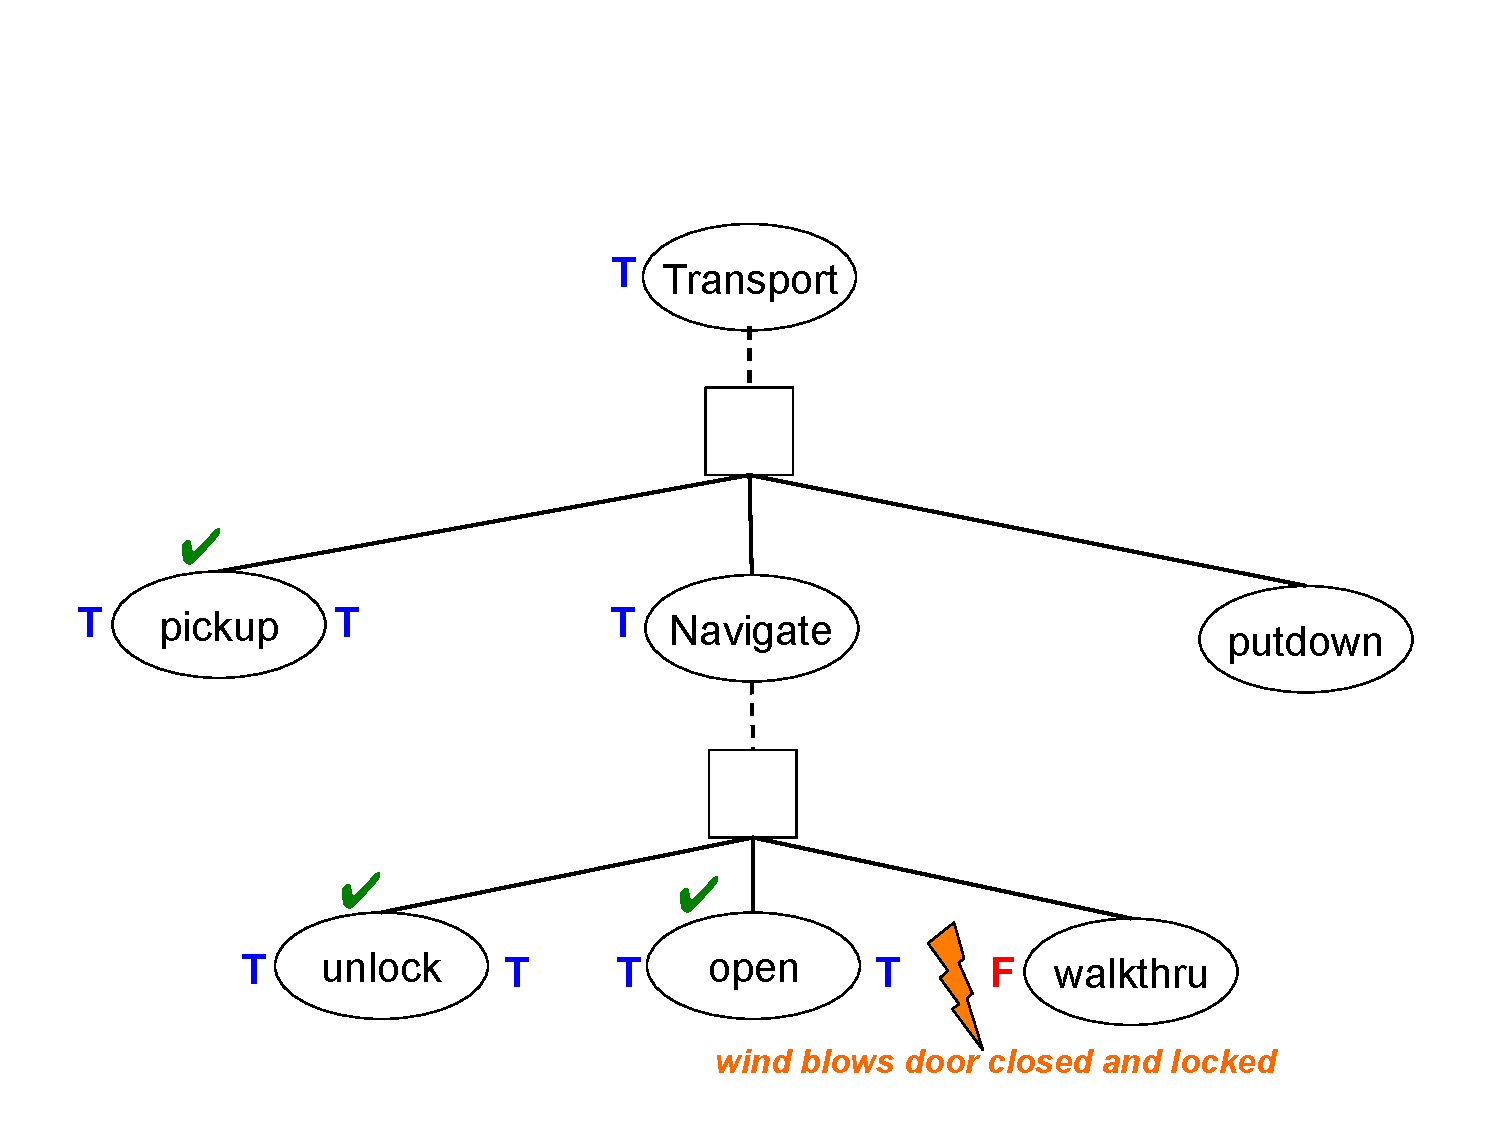
\includegraphics[width=3in]{figs/wind}}
					\vskip 8pt
					\defig{wind}{Cassure dans l'exécution du HTN après que le vent a fait claquer la porte et l'a bloquée. Les coches indiquent les tâches dont l'exécution est terminée. ``T'' représente une condition dont l'évaluation a retourné \emph{vrai}; ``F'' représente une condition qui a retourné \emph{faux}.}
				\end{figure}
	
		\section{Motivations}
		Afin de mieux introduire et expliquer notre travail, nous présentons dans cette section un exemple simple mais intuitif d'une cassure dans l'exécution d'un HTN et sa réparation. L'idée de base de cet exemple, illustré dans la  \fig{recover}, est l'implémentation d'un robot en HTN pour transporter un objet a travers une porte fermée. Dans le HTN, la tâche but {\em transport}, est décomposée en trois étapes: ramasser l'objet ({\em pickup}), manipuler la porte {\em(navigate)} et poser l'object {\em(putdown)}. La tâche {\em navigate} est à son tour décomposée en quatre étapes: déverrouiller  la porte {\em(unlock)}, l'ouvrir {\em(open)} et franchir la porte {\em(walkthrough)}. Chacune de ces tâches est représentée par un ovale dans la figure \fig{wind}. Les boîtes représentent les différentes alternatives de décomposition qui peuvent être ignorées dans cet exemple. Au moment de l'exécution décrit dans la figure \fig{wind}, le robot a ramassé l'objet, déverrouillé et ouvert la porte avec succès. Cependant, avant que la précondition de la tâche {\em walkthrough} ne soit évaluée, le vent souffle et la porte de ferme et se verrouille (l'exemple ne vise pas à être réaliste mais à illustrer notre propos). La précondition de la tâche {\em walkthrough} évalue si la porte est ouverte et retourne faux. À ce moment, aucune tâche ne peut être exécutée dans le HTN et c'est ce que nous appelons une {\em cassure}. Il n'est pas rare qu'un HTN réactif rencontre des cassures, spécialement dans le cas d'exécution dans des environnements dynamiques et complexes. Cependant, en analysant la cassure produite dans cet exemple, la solution montrée dans la \fig{recover} parait évidente: déverrouiller la porte et l'ouvrir. Par ailleurs, trouver une solution pour cette cassure est un problème triviale pour un planificateur linéaire symbolique comme STRIPS si les (pré/post)conditions des tâches primitives correspondantes étaient spécifiées symboliquement (ce qui n'est pas le cas dans un HTN réactif).
		
			\begin{figure}[t]
				\centerline{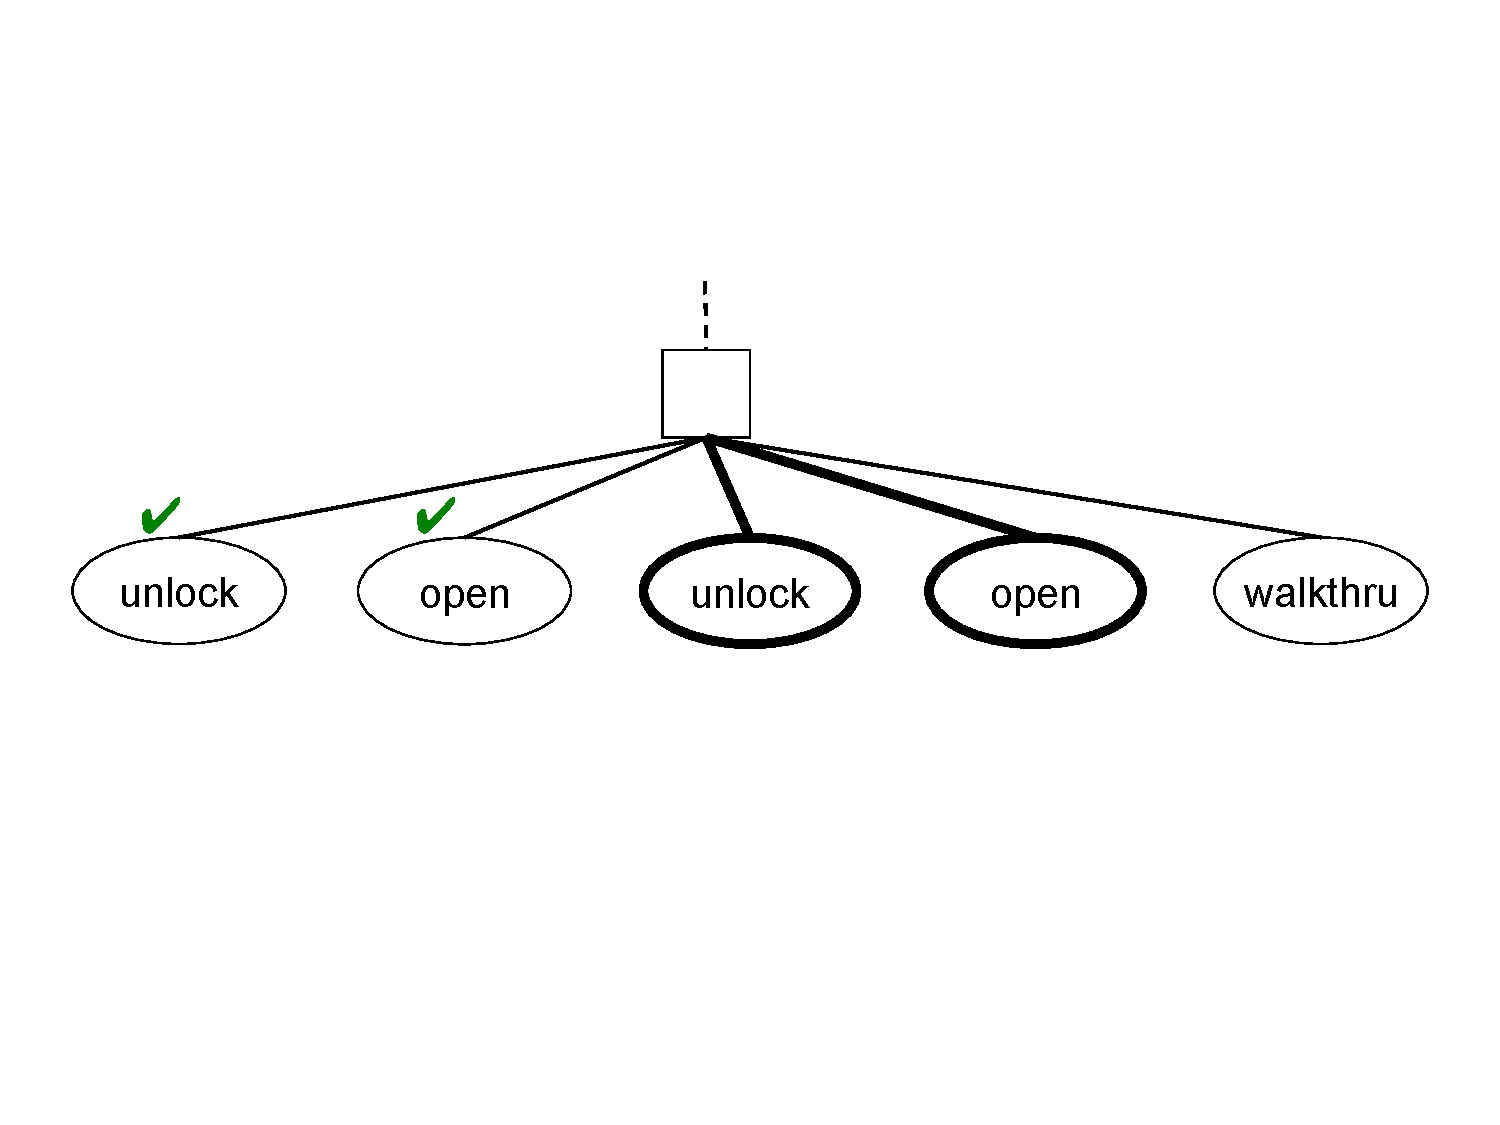
\includegraphics[width=3in]{figs/recover}}
				\vskip 8pt
				\defig{recover}{Suite de deux tâches primitives (en gras) ajoutées au plan hiérarchique de la tâche ``navigate'' pour réparer la cassure de la figure~\fig{wind}.}
			\end{figure}
	
%XXXX ICI NICO

	
		\par Dans les HTN réactifs, pré-et postconditions sont définies en langage  procédural et évalués par un interpréteur approprié à ce langage. \fig{procedures}  montre les  conditions procédurales définies dans le plan {\em Navigate} comme elles seraient typiquement écrites par exemple en JavaScript. 
	%	Prenons  l'exemple de la procédure ``isOpen()'' qui appelle un code spécifique dan le système de capteurs du robot pour évaluer si la porte est actuellement ouverte.
		 En comparaison, \fig{features} montre la formalisation symbolique  des mêmes tâches primitives en STRIPS. 
		Supposons que lorsque la cassure a était détectée dans \fig{wind}, le moteur d'exécution du HTN  contenait la connaissance symbolique qui est dans la  \fig{features}. La réparation de la cassure pourrait donc être traitée comme une problème de planification STRIPS (voir \fig{planning}) dans lequel l'état initial est représenté par l'état courant du monde et l'état final est la précondition échouée de la tâche {\em walkthru} (la porte est ouverte). Un simple chainage arrière peut rapidement trouver une séquence d'actions; à savoir déverrouiller et ouvrir la porte. Le plan produit est ensuite intégré au HTH  comme dans la \fig{recover} et permettre au HTN de reprendre son exécution.  Le but de cet article est de généraliser la solution de cet exemple en algorithme de réparation de cassures qui soit indépendant des applications et auquel on associe une méthodologie de modélisation des HTNs réactifs.
		
		
		\begin{figure}[t]
			\centering
			\begin{subfigure}{2.3in}
				\centerline{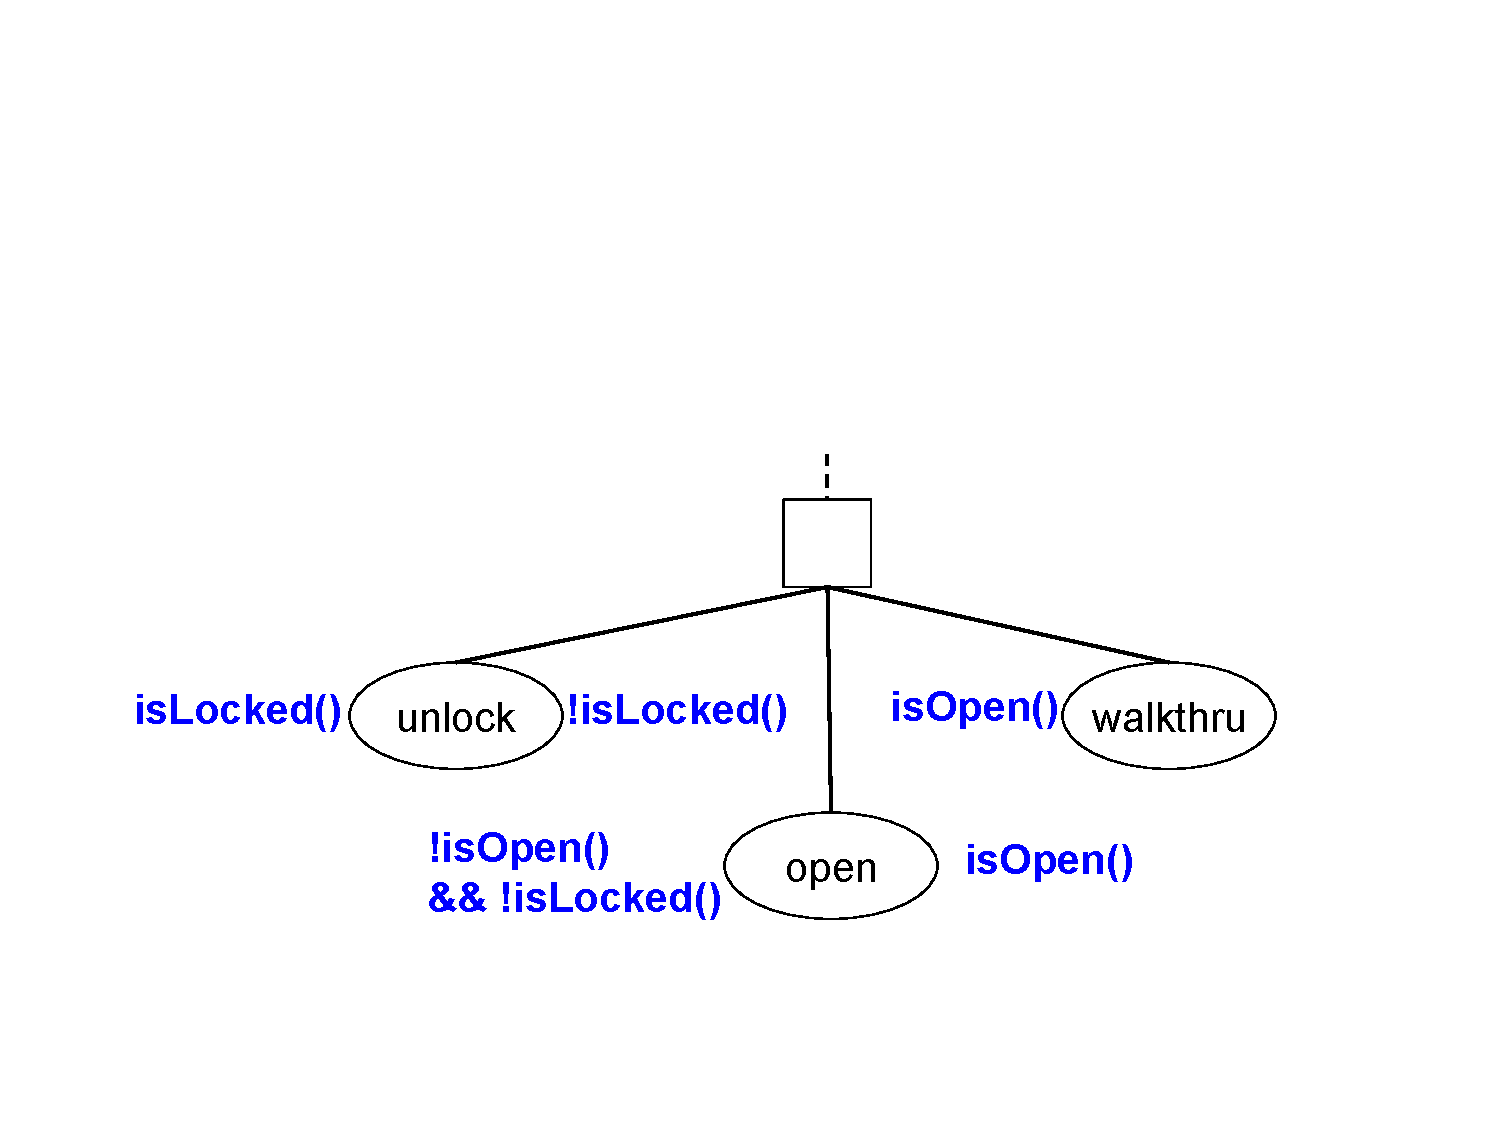
\includegraphics[width=2.4in]{figs/procedures}}
				\vskip 8pt 
				\defig{procedures}{Conditions procédurales }
			\end{subfigure}
			\hfill
			\begin{subfigure}{2.3in}
				\centerline{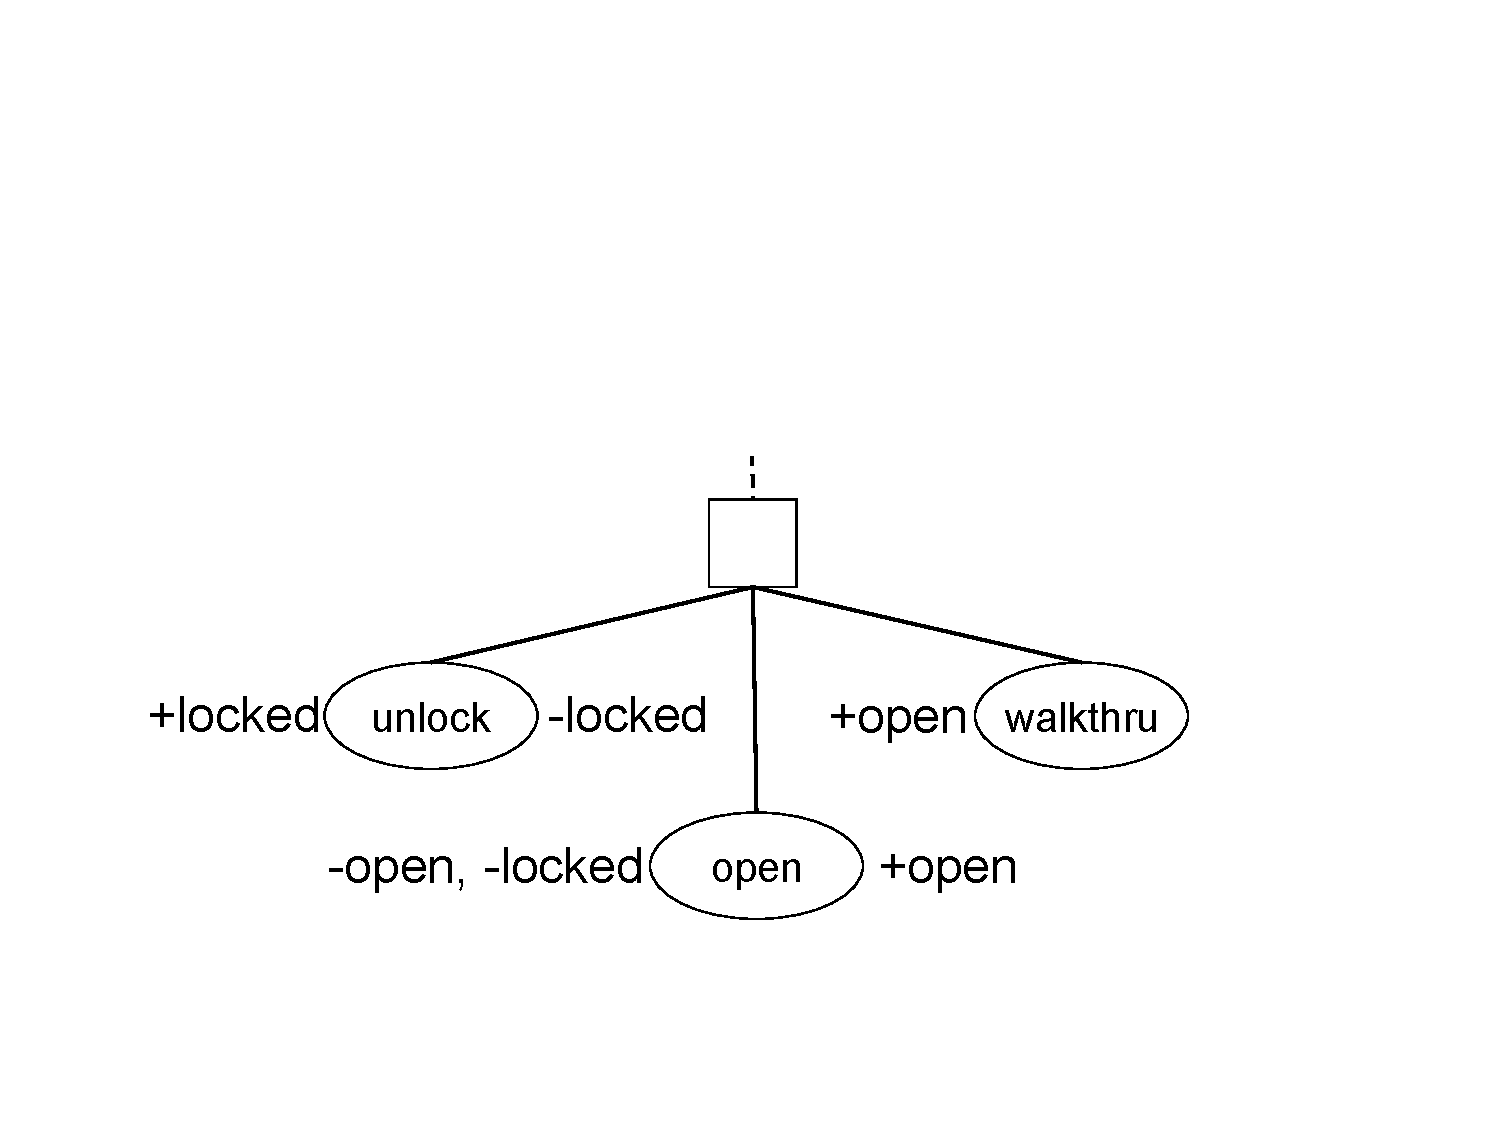
\includegraphics[width=2.4in]{figs/features}}
				\vskip 8pt 
				\defig{features}{Représentation symboliques des conditions}
			\end{subfigure}
			\vskip 8pt
			\defig{comparison}{Conditions procédurales versus symboliques pour le plan Navigate.}
		\end{figure}
		%
		\begin{figure}[]
			\centerline{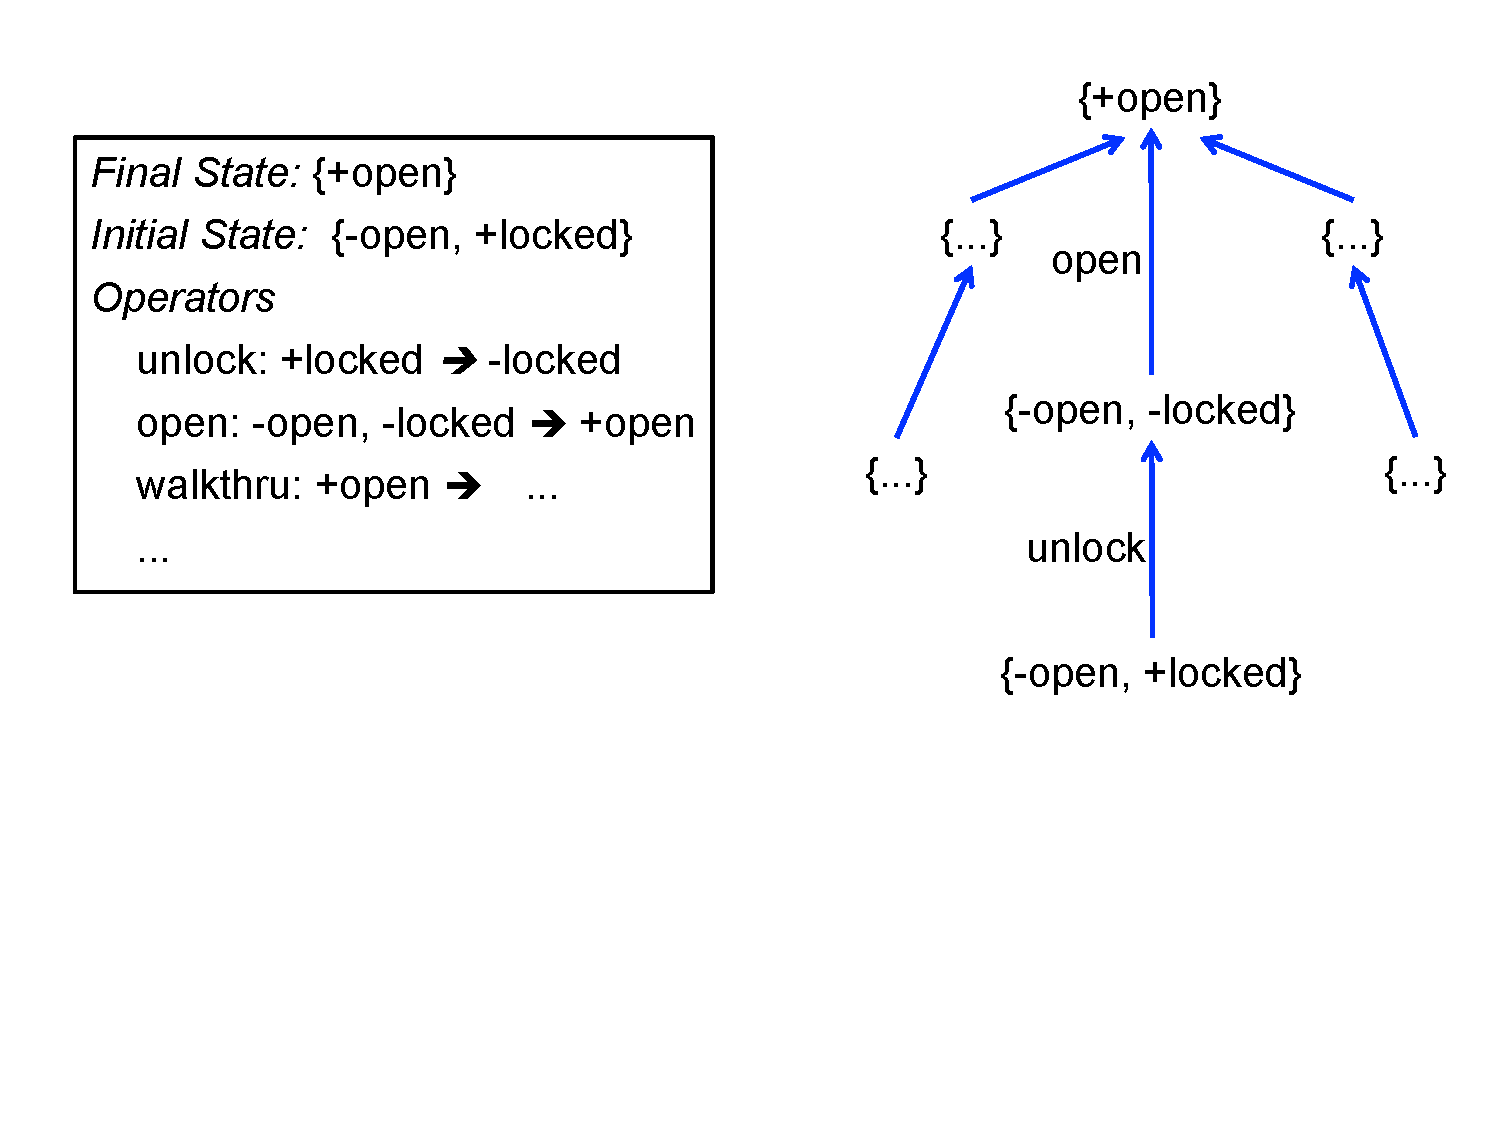
\includegraphics[width=3.7in, height=1in]{figs/planning}}
			\vskip 8pt
			\defig{planning}{réparation de la cassure \fig{wind} comme un problème de planification STRIPS.}
		\end{figure}
		 
		
		\section {Modélisation procédurale VS modélisation symbolique}
		La question que pourrait soulever la section précédente est pourquoi ne pas utiliser seulement la planification symbolique au lieu d'un HTN et appliquer les solutions existantes de réparation des cassure ?. La réponse à cette question mène directement à la problématique de modélisation. En effet, les planificateurs symboliques comme STRIPS requièrent une description  symbolique {\em complète} et {\em correcte} de toutes les tâches primitives dans le domaine du problème. Les différents planificateurs utilisent différentes formalisations pour cela comme le (add/delete) liste dans la \fig{features} ou PDDL \cite{ghallab1998pddl}. Cependant, tous ces planificateurs ont un point  commun, si la description symbolique est incomplète ou incorrecte, alors les plans générés vont subir des cassures. 
		\par Malheureusement, la recherche en IA a monté que la modélisation d'une description logique du monde réel qui soit complète et correcte  peut se révéler extrêmement difficile voir impossible  pour des raisons de fins pratiques.  La difficulté de la modélisation symbolique est la raison principale pour laquelle les HTNs réactifs ont été inventés. La connaissance est insérée dans les HTN réactifs principalement a deux endroits: dans la structure de décomposition de l'arbre et dans le code pour définir les conditions procédurales (spécialement dans les conditions d'applicabilités pour les choix de décompositions). grâce a leur facilité de modélisation les HTNs sont utilisés pour les  problèmes de domaines complexes. En effet, il est bien connu que l'architecture hiérarchique facilite aux personnes l'organisation de leur pensées et leur permet de faire face à la complexité des tâches. De plus, les conditions procédurales comme une précondition n'est évaluée que dans l'état {\em courant} du monde, quant aux descriptions symboliques, elle doivent être vrais dans tous les mondes possibles. Ceci dit les HTNs réactifs rencontrent des cassures, ce qui nous a mené à proposer notre solution; à savoir une approche hybride dans laquelle un HTN réactif est augmenté avec de la connaissance symbolique afin d'aider à la réparation des cassures. 
		
		\section{L'approche hybride}
		Dans cette section, nous proposons une généralisation sur deux niveaux de l'exemple de la section 2 en considérant: (1) les différents types de cassures, (2) l'ensemble des états finaux possibles. Nous présenterons d'abord l'algorithme général de réparation de cassure et discuterons ensuite méthodologie de modélisation associée.
			\begin{figure*}[t]
				\centering
				\begin{subfigure}{2.1in}
					\centerline{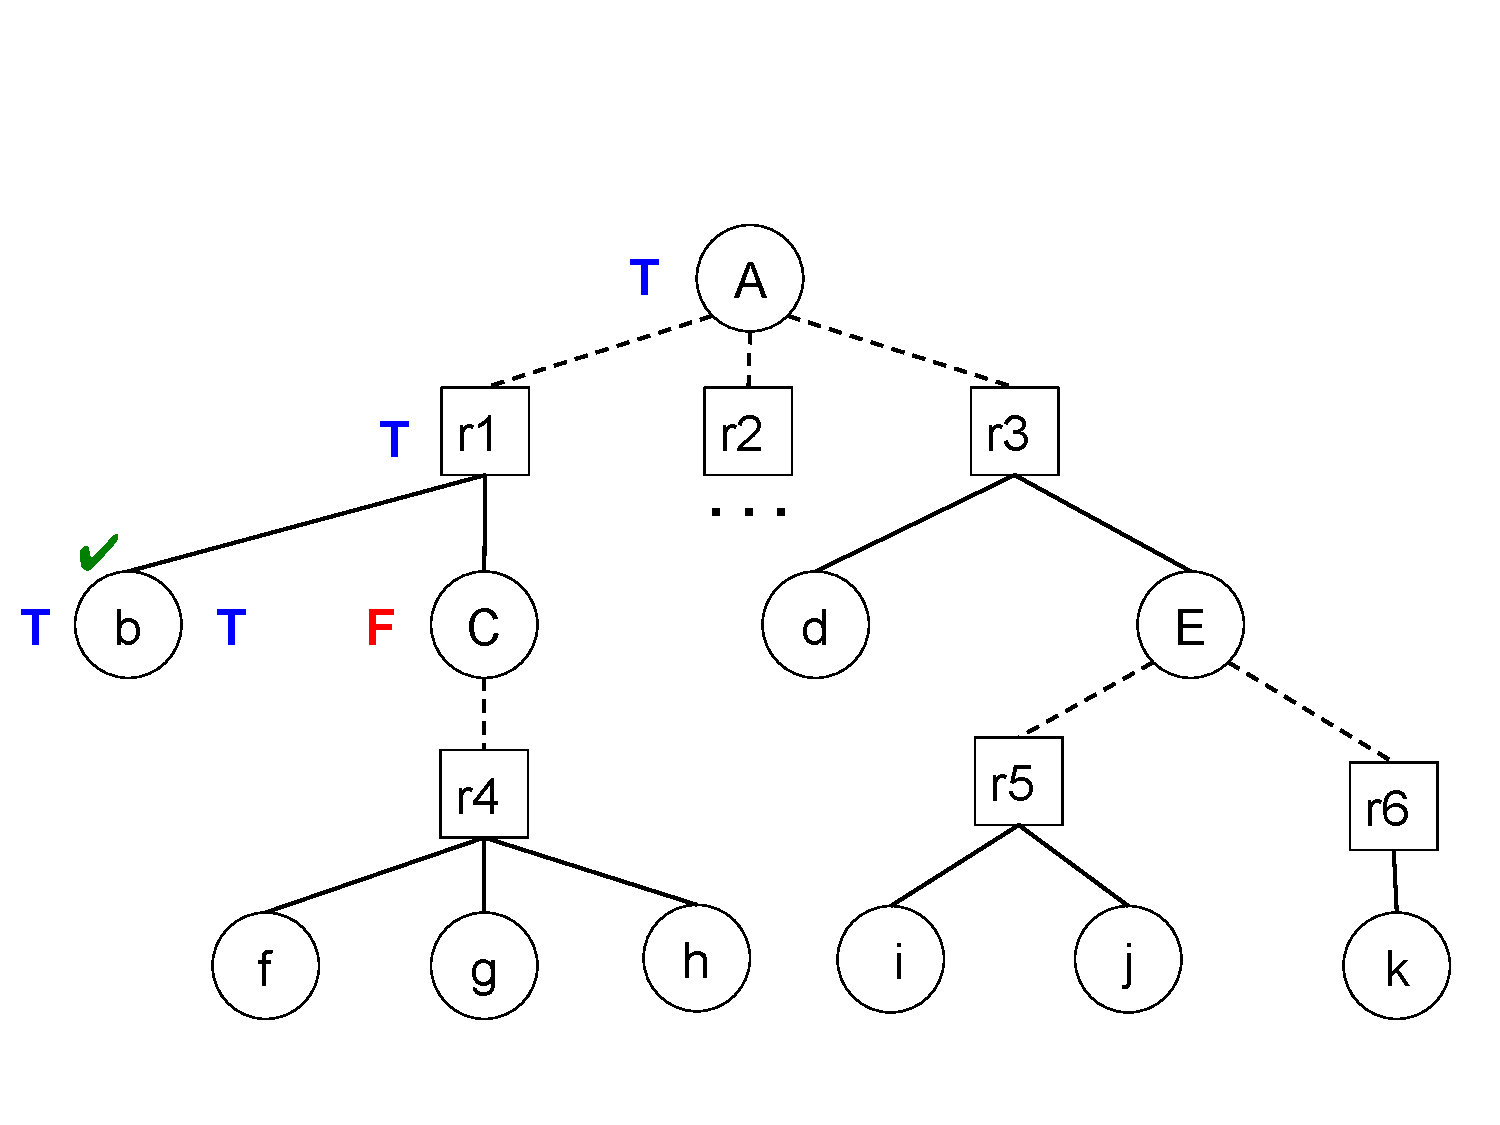
\includegraphics[height=1.3in]{figs/precondition}}
					\vskip 8pt 
					\defig{precondition}{précondition échouée}
				\end{subfigure}
				\hfill
				\begin{subfigure}{1.4in}
					\centerline{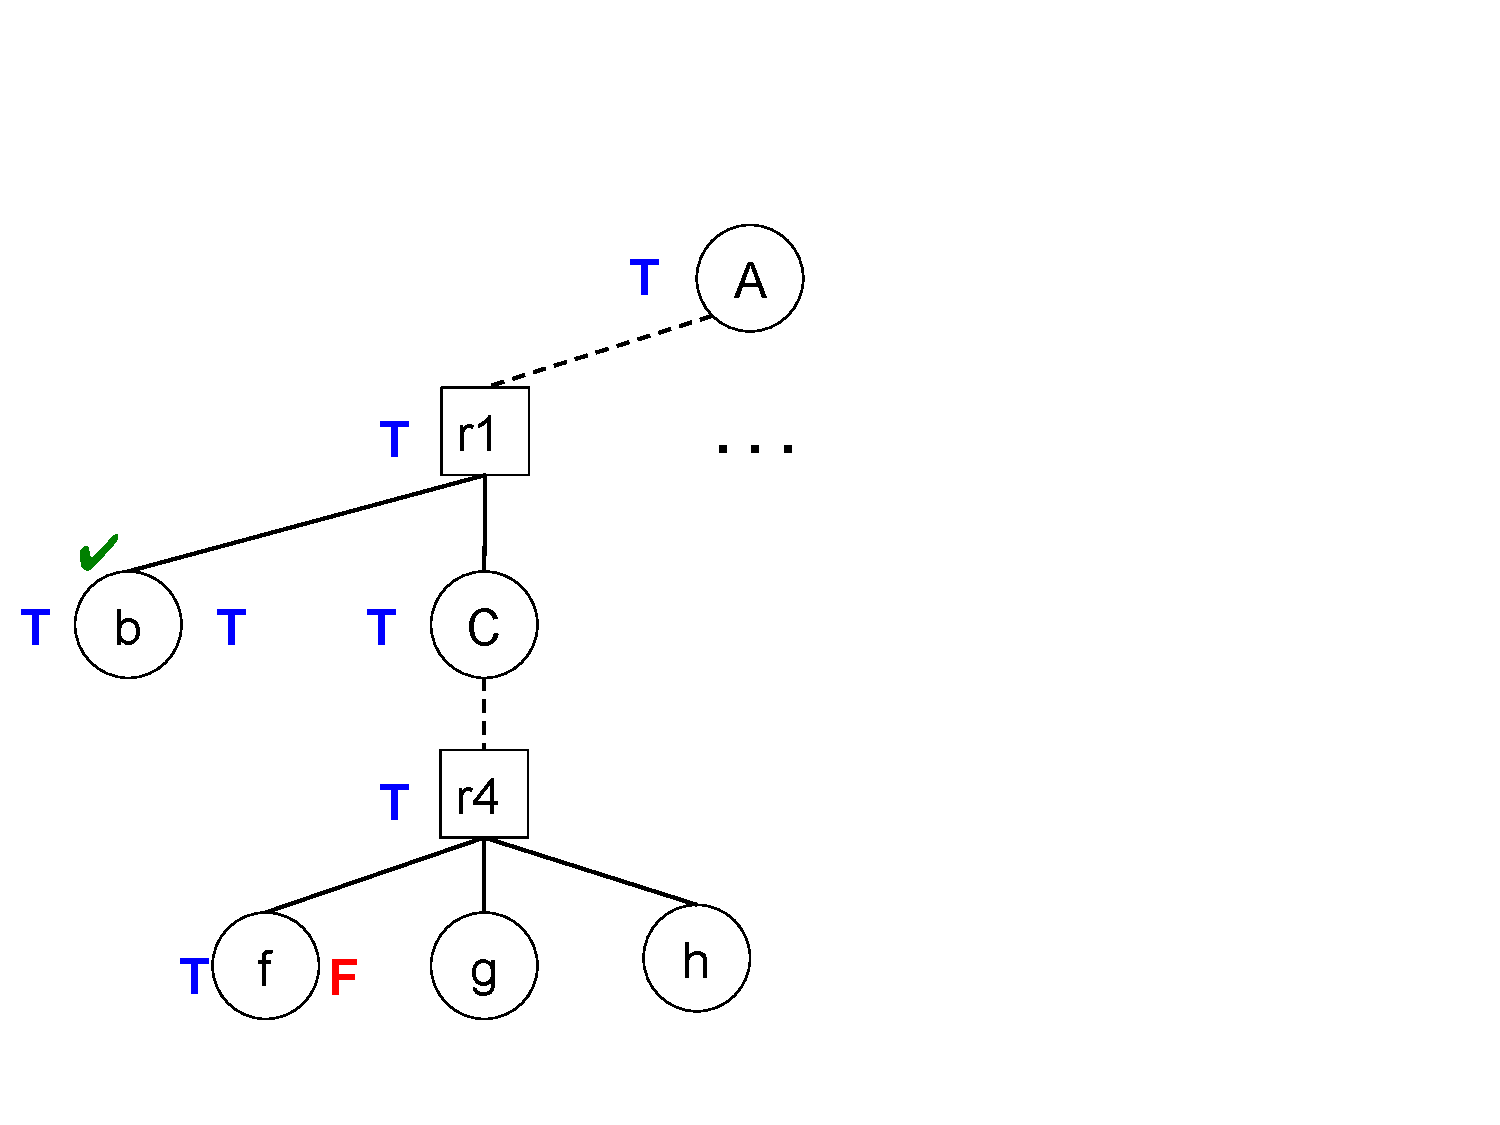
\includegraphics[height=1.3in]{figs/postcondition}}
					\vskip 8pt 
					\defig{postcondition}{postcondition échouée}
				\end{subfigure}
				\hfill
				\begin{subfigure}{1in}
					\centerline{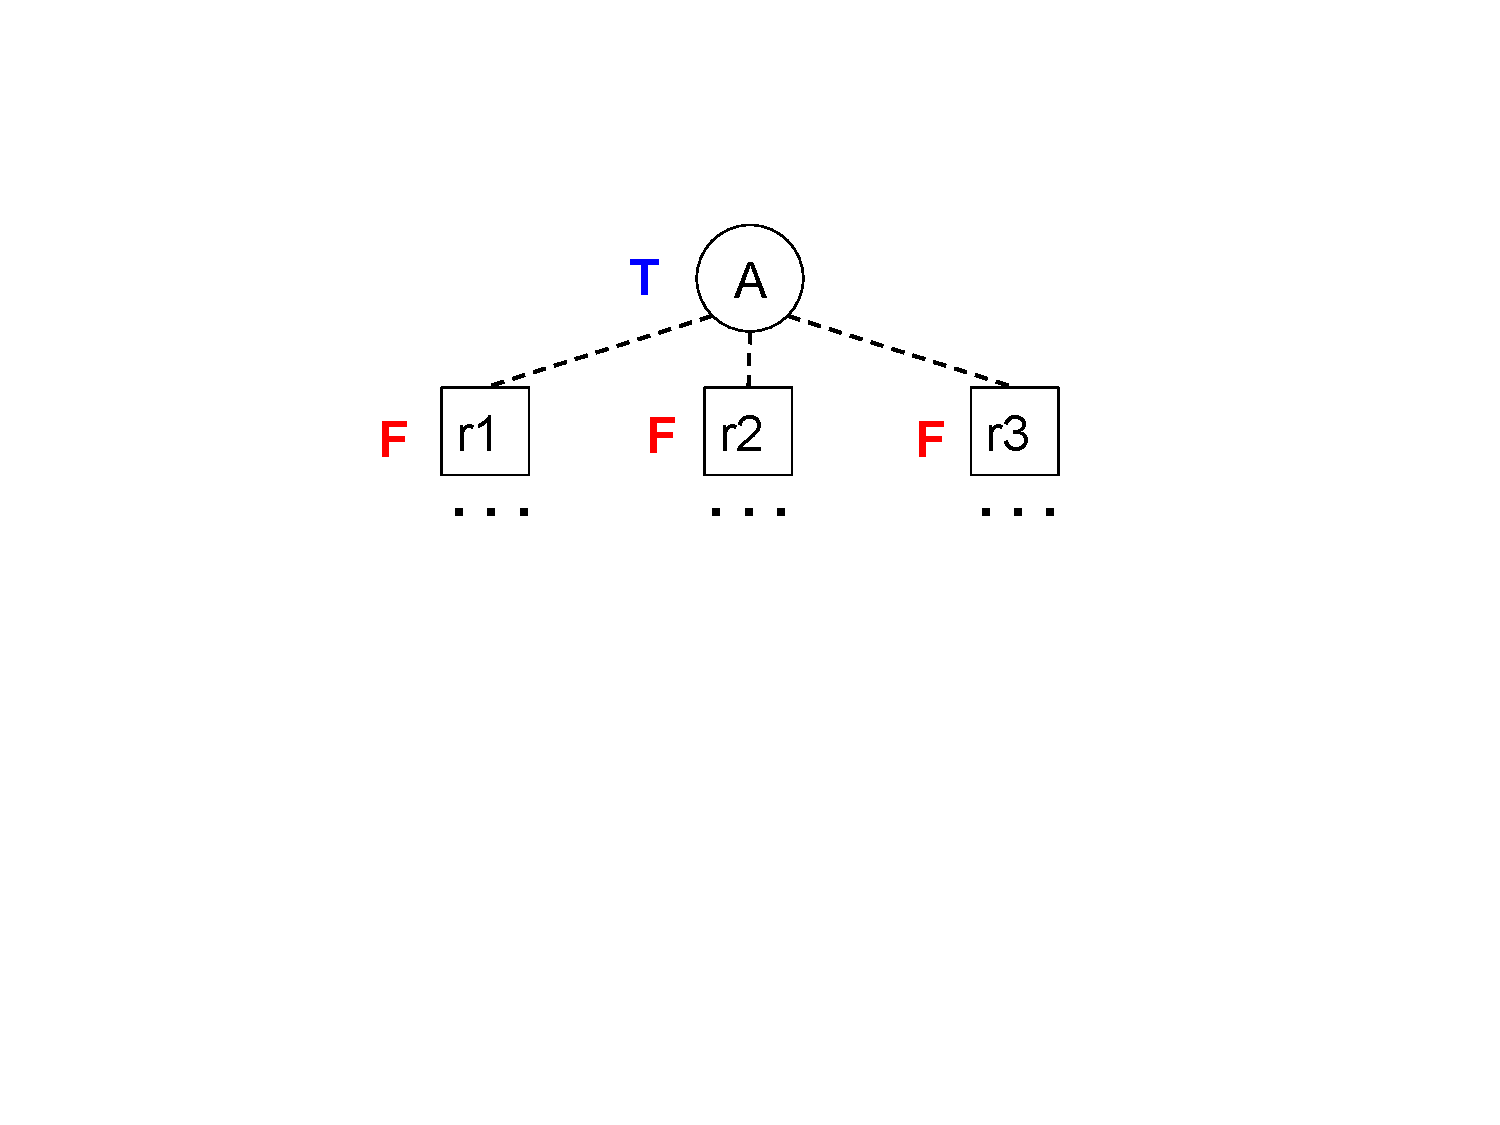
\includegraphics[height=1.3in]{figs/applicability}}
					\vskip -2pt
					\defig{applicability}{condition d'applicabilité échouée}
				\end{subfigure}
				\vskip 4pt 
				\defig{breakdowns}{Examples of the three types of breakdown in reactive HTN execution.} 
			\end{figure*}
			
		\subsection{Les HTNs réactifs}
		Un HTN réactif est un arbre biparti avec  différents niveaux de  n\oe uds {\em tâches} et   n\oe uds {\em décompositions}. Il est définit avec un n\oe ud tâche à la racine et aux feuilles. Ces dernières sont appelée {\em tâches primitives} et les autres sont appelées {\em tâches abstraites}. Les n\oe uds de l'arbre sont associés avec trois types de procédures booléennes, chacune étant évaluée uniquement dans l'état courant. Les nœuds tâches sont définis avec des {\em pré/postconditions} optionnelles et chaque nœud de décompositions a une {\em condition d'applicabilité}.
		\par Les HTNs réactifs peuvent être représentés comme un arbre et/ou, où les tâches sont des "et", et les nœuds de décomposition sont des "ou". L'exécution est en profondeur d'abord, avec un parcours de gauche à droite à partir du nœuds racine, durant lequel les conditions sont évaluées, comme décrit dans la suite. 
		\par Si l'exécution du nœud courant est une tâche alors ses éventuels préconditions sont évaluées. si elle retournent faux, alors l'exécution est interrompue (cassure); sinon l'exécution continue. Si la tâche est primitive, elle est directement exécutée pour changer l'état du monde. Sinon si elle est abstraite alors les conditions d'applicabilités des nœuds fils (décompositions) sont évalués dans l'ordre jusqu'à l'obtention d'un nœud qui retourne vrai. L'exécution continue alors avec cette décomposition. Si toutes les conditions d'applicabilités sont fausses alors  l'exécution est arrêtée(cassure). Une fois l'exécution de la tâche terminée, ses éventuelles postconditions sont évaluées, si elles retournent faux alors l'exécution est interrompue (cassure). Sinon l'exécution continue. Si le nœud courant étant exécuté est une décomposition, alors les nœuds fils (tâches) sont exécutées dans l'ordre. 
		\par La \fig{breakdowns} résume les trois types de cassures qu'un HTN peut rencontrer durant son exécution. La cassure dans l'exemple de la section 2 est causé par une précondition échouée. Cependant, cette taxonomie n'est pas apte à distinguer les raisons sous-jacentes possibles qui causent des cassures. En effet, une cassure peut être causée par un changement inattendu dans le monde (ex: le vent dans la section 2); ou a cause d'une erreur de programmation (condition mal codée, structure d'arbre erronée). L'impossibilité de détecter les causes des cassures est une limitation intrinsèque des HTN réactifs.
		
			\subsection{Algorithme de réparation de plans}
			\noindent Le généralisation la plus significative de l'algorithme sur l'exemple de la Section 2, concerne le choix de l'état final pour le planificateur linéaire. Cependant, pour ce même exemple, différents état buts peuvent être trouvés.  Par exemple, supposons que {\em walkthru} ait une postcondition qui spécifie que le robot est dans la pièce à l'autre côté de la porte. Donc, après la cassure, le robot peut trouver une autre méthode de réparation; trouver un plan pour satisfaire cette postcondition. (ex, sortir de la pièce actuelle par une autre porte, passer par autre chemin pour la pièce de destination). Cette procédure consiste à définir la postcondition comme {\em le but} d'un  des candidats pour la réparation. De la même façon, supposons que {\em walkthru}n'a pas de représentation symbolique pour sa postcondition, mais la postcondition symbolique de {\em navigate} spécifie la location bute du robot. Dans ce cas la postcondition de {\em navigate} est considérée comme un état but de réparation. Il est a noté que les conditions d'applicabilités sont un cas a part pour le calcul des candidats. En effet, une condition d'applicabilité est considérée comme candidat dans l'unique cas où toutes ses sœurs dans l'arbre ont été évaluées comme fausses.
			L'idée est de construire l'ensemble des candidats le plus général possible qui inclut toutes les conditions du HTN qui n'ont pas déjà étaient validées durant l'exécution. Cette approche pourrait être excessivement générale, mais requière  plus d'expérience pour construire une meilleure. 
			\par \fig{pseudo} présente le pseudo code du système hybride conçu. Le procédure principale, {\sc Execute}, execute un HTN jusqu'à ce qu'il retourne soit succès soit une cassure est détectée. Le code de réparation de cassure commence à la ligne 5. La sous procédure, {\sc FindCandidates}, va récursivement parcourir le HTN afin de calculer les candidats cibles pour la procédure de réparation. La procédure {\sc SymbolicPlanner} n'est pas décrite car n'importe quel planificateur linéaire peut être utilisé. De plus, comme l'ensemble des opérateurs symboliques ne change pas durant l'exécution, Il n'est donc définit comme un argument explicite au planificateur symbolique.(voir section 4.3). 
			
			\par Plus en détail, on peut voir à la linge 6 que notre approche requière une méthode pour calculer,  à partir de l'état courant, l'état initial du planificateur symbolique dans un  formalisme symbolique que le planificateur puisse exploiter. Par exemple, pour le planificateur dans la section 2, chaque fonction symbolique comme ``open'' doit être associée à une procédure comme ``isOpen()'' afin de pouvoir calculer sa valeur dans l'état courant. Cette association est une des parties de la modélisation hybride de notre modèle (voir partie 4.3 pour plus de détails). La ligne 8 montre que les candidats sont triés par rapport à leurs distance au nœud courant dans l'arbre, en utilisant une simple métrique (Ex: le plus court chemin dans un arbre non dirigé). La raison principale est de favoriser des réparations locale qui  préservent au maximum  la structure originale du HTN. Cependant, nous n'avons pas encore testé les performances de cette heuristique. 
			Finalement, à la ligne 12 de la procédure {\sc execute}, quand un plan est trouvé il doit être intégré dans le HTN. La difficulté de cette étape réside dans la distance entre le premier et le dernier nœud. Plus ces derniers sont distants plus les changement  devant être effectués dans la structure du HTN sont compliqués 
		\begin{figure}[t]
		
			\begin{algorithmic}[1]\small
				
				\Procedure{Execute}{$htn$}
				\While{$htn$ is not completed} 
				\State $current\gets$ next executable node in $htn$
				\If{$current\neq null$} execute $current$
				\Else\hskip 0.1in [breakdown occurred]
				\State $initial\gets$ symbolic description of current world state
				\State $candidates\gets FindCandidates(htn)$
				\State sort $candidates$ by distance from $current$
				\For{$final \in candidates$}
				\State plan$\gets$ SymbolicPlanner(initial,final)
				\If{$plan\neq null$}
				\State splice $plan$ into $htn$ between $current$ and $final$
				\State \textbf{continue} while loop above
				\EndIf
				\EndFor
				\State Recovery failed!
				\EndIf
				\EndWhile
				\EndProcedure
				\Statex
				\Procedure{FindCandidates}{$task$}
				\State $conditions\gets\emptyset$
				\State $pre\gets$ symbolic precondition of $task$
				\If{$pre\neq null\;\wedge$ procedural prec of $task$ has not evaluated to true}
				\State add $pre$ to $conditions$\EndIf
				\State $post\gets$ symbolic postcondition of $task$
				\If{$post\neq null\;\wedge$ procedural postc of $task$ has not evaluated to true}
				\State add $post$ to $conditions$
				\EndIf
				\State $applicables\gets\emptyset$
				\State $allFalse\gets true$
				\For{$decomp \in$ children of $task$}
				\For{$task\in$ children of $decomp$} $FindCandidates(task)$
				\EndFor 
				\If{$allFalse$}
				\If{procedural appl condition of $decomp$ has evaluated to false}
				\State $app\gets$ symbolic applicability condition of $decomp$
				\If{$app\neq null$} add $app$ to $applicables$\EndIf
				\Else $\;allFalse\gets$ false
				\EndIf 
				\EndIf
				\EndFor
				\If{$allFalse$} add $applicables$ to $conditions$
				\EndIf
				\State\Return $conditions$
				\EndProcedure 
				
			\end{algorithmic}
			\vskip 8pt
			\defig{pseudo}{Pseudocode de l'exécution et réparation du système HTN réactif hybride}
		\end{figure} 
		\subsection{Méthodologie de modélisation}
		Le système hybride prend avantage de la connaissance symbolique construite par l'auteur du HTN, sachant que toute condition  dans le HTN peut, ou non, avoir une représentation symbolique. Comme  nous l'avons exposé précédemment, la difficulté liée à la réalisation d'une modélisation symbolique a mené les auteurs des HTNs à utiliser la modélisation procédurale. Il existe donc deux problèmes méthodologique liées à la conception d'un HTN hybride;  d'une part, il faut situer où il est préférable d'investir et l'effort à consacrer pour la modélisation symbolique. D'une autre part, Il faut définir une stratégie qui facilite à l'auteur le processus de mixage entre le procédural et le symbolique. Notre intuition primaire consiste à réduire la modélisation symbolique aux tâches primitives, car nous espérons que l'utilisation d'une stratégie locale pour la réparation des cassures soit plus efficace. Le choix des opérateurs à introduire au planificateur linéaire ont une implication directe sur ses performances. En effet, seules les tâches primitives disposant d'une représentation symbolique de ses pré et postconditions peuvent être inclut dans l'ensemble des opérateurs. Cependant, si une tâche abstraite dispose de ses caractéristiques, elle peut alors être  utilisée pour la réparation des cassures, en utilisant durant son exécution une de ses décompositions étant valables dans l'état courant. 
		\par Nous proposons de mettre en œuvre un outils qui aiderait à réduire la complexité de le modélisation hybride, qui pourrait reconnaitre les conventions entre les deux modélisations comme dans la \fig{procedures} et automatiquement générer sa représentation symbolique comme dans la   \fig{features}. Il peut aussi garder l'historique des cassures et les utiliser pour conseiller l'auteur où il devrait ajouter des connaissances symboliques dans le HTN.
	\section{Implémentation et évaluation}
	Nous avons implémenté notre système hybride en Java.en utilisant le standard ANSI/CEA-2012 \cite{rich2009building} pour la modélisation du HTN et Disco \cite{rich2012using} comme le moteur d'exécution du HTN. Concernant le planificateur symbolique, nous avons utilisé une simple implémentation de STRIPS  exécutée dans un environnement Java de Prolog\footnote{See http://tuprolog.apice.unibo.it}. L'utilisation de Prolog facilite l'ajout de règles de raisonnement symboliques durant le processus de planification. 
	\par L'évaluation ultime de notre approche consiste à faire évoluer plusieurs agents dans des environnements dynamiques du monde réels et évaluer leur performances ainsi que leur robustesses face aux cassures. Entre temps, nous avons validé notre système avec une évaluation préliminaire sur des HTNs générés synthétiquement en variant le niveau de connaissance symbolique. Nous sommes partis d'une théorie simple qui dit plus il y'a des connaissances symboliques dans le HTN, mieux seront ses performances pour la réparation des cassures. 
		\fig{results} montre les résultats obtenus qui confirment notre hypothèse. Nous avons testé deux configuration d'HTNs RxSxD, 3x3x3 et 1x5x4, où R est le facteur de ramification d'une décomposition (recipe), S le facteur de ramification d'une tâche, D étant la profondeur du HTN.  Pour chaque test, nous avons aléatoirement extrait toutes les combinaisons possibles de connaissance symbolique sur trois différent niveaux; 25\% , 50\%, 75\% (le pourcentage des conditions qui ont une représentation symbolique). Nous nous sommes restreints à ces modélisations pour des questions de temps d'exécutions. 	\fig{recovery} montre l'évolution des performances de réparations de cassures en fonction du l'augmentation du niveaux de connaissance symbolique. Dans la fig{results}, nous nous sommes intéressés à la proportions des problèmes de planifications soumis au planificateur (buts candidats) qui ont été correctement résolu augmente aussi en fonction du niveaux de connaissance symbolique. (Pour ces tests, nous avons modifié notre systèmes pour qu'il génère un plan pour tous les candidats).
		\begin{figure}[t]
			\centering
			\begin{subfigure}{2.3in}
				\centerline{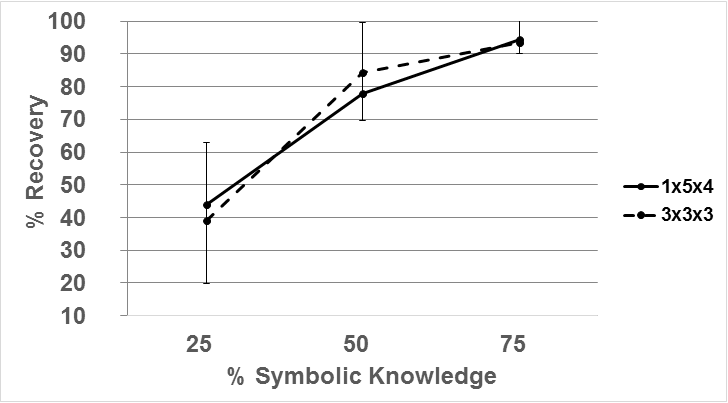
\includegraphics[width=2.3in]{figs/recovery}}
				\vskip 8pt 
				\defig{recovery}{Ration des réparation/cassure}
			\end{subfigure}
			\hfill
			\begin{subfigure}{2.3in}
				\centerline{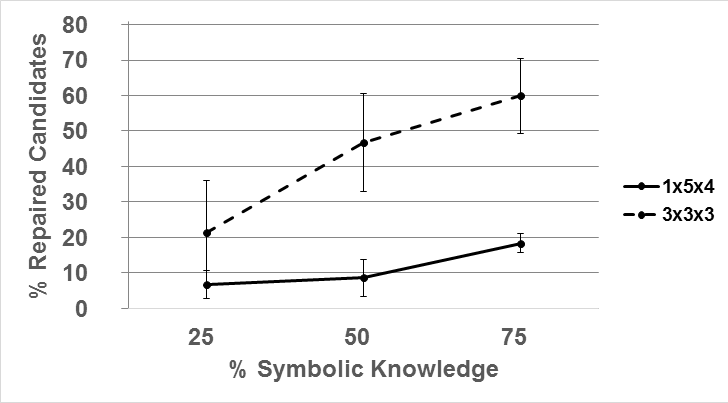
\includegraphics[width=2.3in]{figs/candidates}}
				\vskip 8pt 
				\defig{candidates}{Proportion des candidats réparés}
			\end{subfigure}
			\vskip 6pt
			\defig{results}{Résultats des expérimentations sur des HTNS générés synthétiquement avec différents niveaux de connaissances symbolique.}
		\end{figure}
\section{Conclusion}
 Nous avons présenté dans cet article notre contribution pour la réparation des cassure qui consiste à augmenter un HTN réactifs avec un planificateur linéaire symbolique qui propose des plans de réparations. Nous avons ensuite soulevé la question sous-jacente à la modélisation hybride de notre système et expliquer le compromis existant entre la modélisation symbolique et procédurale. Une implémentation en Java a été proposé qui combine un HTN réactif appelé Disco et le planificateur STRIPS implémenté en Prolog. Des tests sur des HTNs synthétiques ont été mené pour valider le système et les résultats obtenus confirment nos théories de départ.  Des futures perspectives sont envisagées. En effet, un travail de thèse est entamé qui consiste à intégrer notre modèle dans un système de dialogue social afin de gérer de manière opportuniste les éventuelles cassures.  
	% ====================================================================					
		\vskip 4pt
		\bibliographystyle{plain}
				\bibliography{bibliography} % The references (bibliography) information are stored in the file named "Bibliography.bib"
							
				\end{document}
				
				
